%Define all the package in this document
\documentclass{article}
\usepackage[utf8]{vietnam}
\usepackage{amsmath} 
\usepackage[⟨options⟩]{fancyhdr}
\usepackage[a4paper, total={6in, 9in}]{geometry}
\usepackage{graphicx} % Required for inserting images
\usepackage[]{mdframed}

\title{Sequences and Series}
\author{USTH Learning Support }
\date{December 2023}

\begin{document}

\maketitle

\tableofcontents

\pagebreak
%
%Phan 1: Sequences, cac van de lien quan toi sequences. 
%
\section{Sequences}
\subsection{Definitions}
%
%Định nghĩa Sequence
%
\textit{Sequences} are things from which series are built. A sequence is nothing but an infinite list of numbers, written in \textbf{a definite order}: $$ a_1, a_2, a_3, a_4,...$$
To say a sequence \textit{converges} to a number L is to say that the terms of the sequence get closer and closer to L the further along the sequence we go. Written in terms of limits, we have: 
$$ \lim_{n\to\infty} a_n = L$$
A sequence \textit{diverges} just means that it does not converge. Let's take a look at some examples:
%
%Example 1   Sequences
%
\begin{enumerate}
    \item Consider the sequence: $$a_n = 2 + \frac{(-1)^n}{n^2}$$
    The first few terms of this sequence are: $$ 2 + \frac{-1}{1^2}, 2 + \frac{1}{2^2}, 2 + \frac{-1}{3^2}, 2 + \frac{1}{4^2}, ... $$
    As $n$ goes to infinity, the $\frac{(-1)^n}{n^2}$ gets closer and closer to zero, since the numerator bounces     back forth between $-1$ and $1$ while the denominator gets larger and larger. Thus: 
    $$\lim_{n\to\infty} a_n = \lim_{n\to\infty} \left(2 + \frac{(-1)^n}{n^2}\right) = 2 + 0 = 2$$
    We conclude this sequence converges to 2. 
    %
    %example 2 sequences
    %
    \item Consider the sequence: $$a_n = \frac{2\cdot3^{n+1}}{5^n} + \frac{(3n-1)!}{(3n+1)!}$$
    We can rewrite the first part of the sum as: $$\frac{2\cdot3^{n+1}}{5^n} = \frac{2\cdot3\cdot3^n}{5^n} = 6\left(\frac{3}{5}\right)^n$$
    Observe that this sum converges to 0, as when $n$ gets larger, $\left(\frac{3}{5}\right)^n$ gets smaller and smaller. Thus: 
    $$\lim_{n\to\infty} \frac{2\cdot3^{n+1}}{5^n} = \lim_{n\to\infty} 6\left(\frac{3}{5}\right)^n = 0 $$
    Now, the second part of the sum in the definition of $a_n$ can be written as: 
    $$\frac{(3n-1)!}{(3n+1)!} = \frac{(3n-1)!}{(3n+1)(3n)(3n-1)!} = \frac{1}{(3n+1)(3n)}$$
    It is clear that: 
    $$\lim_{n\to\infty}\frac{(3n-1)!}{(3n+1)!} = \lim_{n\to\infty}\frac{1}{(3n+1)(3n)} = 0 $$
    Since both parts of the sum in the definition of $a_n$ individually converge, we can say that: 
$$\lim_{n\to\infty} a_n = \lim_{n\to\infty} \left(\frac{2\cdot3^{n+1}}{5^n} + \frac{(3n-1)!}{(3n+1)!}\right) = \lim_{n\to\infty} \frac{2\cdot 3^{n+1}}{5^n} + \lim_{n\to\infty}\frac{(3n-1)!}{(3n+1)!} = 0 + 0 = 0 $$ 
so, our given sequence $a_n$ converges to 0.
 \end{enumerate}
 %
 %phan sau: các cách define a sequence (4 phưong pháp)
 %
\subsection{Define a sequence}
Some different ways to define a sequence include: 
\begin{enumerate}
    \item Sequences can be defined by giving a formula for the $n^{th}$ term.
    $${(-1)^n}^{\infty}_{n=1} = {-1, 1, -1, 1}: a_n = (-1)^n$$
    \item Sequences may be defined by different expressions for different subsets of indices (like piece-wise functions). 
    $${c_n} \text{, with } c_n = \left\{\begin{matrix}
1 & 1 \leq n \leq 100  \\
\ln (\sqrt{n} - 10) & n \geq 101 \\
\end{matrix}$$
    \item Sequences may be defined recursively: The Fibonacci sequences $F_1 = F_2 = 1 , F_n = F_{n-1} + F_{n-2} $
    \item Some sequences do not have a simple defining expressions. Example: The sequence ${p_n}$, where ${p_n}$ is the n-th prime number. 
\end{enumerate}
\textbf{Why learn this?} One type of question that may appear in the test is: Determine whether a sequence diverges/converges, but a sequence is not given in the form of the $n^{th}$ term but in the recursive method, for example. It is important that you can try to work that out. Furthermore, we will soon define the convergence property of series based on that of sequence, so you should understand, to the least, what does "the convergence of a sequence" actually mean!\\ \\
\textit{Exercise 1: Can you define the sequence of all positive even integers using the four aforementioned methods?} \\ \\
\textit{Exercise 2: Define a sequence $x_1, x_2, x_3, x_4...$} by setting $x_1 = \sqrt{2}$ and then recursively defining each other term in terms of the previous one via: 
$$ x_{n+1} = \sqrt{2 + x_n} \text{ for } n \geq 1$$
Given that this sequence does diverge,  can you find where does it converge to?
\subsection{More on Divergence and Convergence}
\subsubsection{A formal definition - You can skip it!}
(Feel comfortable to skip this - I only include for those who are "curious"!) \newline \newline 
A sequence is convergent if and only if for every $ \epsilon > 0 $, there exists a number $N$ so that for every $m, n \geq N$, $|a_{m} - a_{n}| < \epsilon$.
\newline 
\newline 
\textbf{Remark:} This is quite similar to the notion of limits. In most textbooks for pure Mathematics guys, Sequences are often discussed before the notion of Limits, Differentiations and Integration. You can verify it by checking "Principles of Mathematical Analysis" by Walter Rudin (famously known as the "Baby Rudin" book - it's not easy as the "baby" title may sound :)). 
\subsubsection{Properties of limits}
As we can define a sequence with the idea of a limit, it is possible that the properties of limits also apply to the properties of a sequence. Let's review this: 
\begin{center}
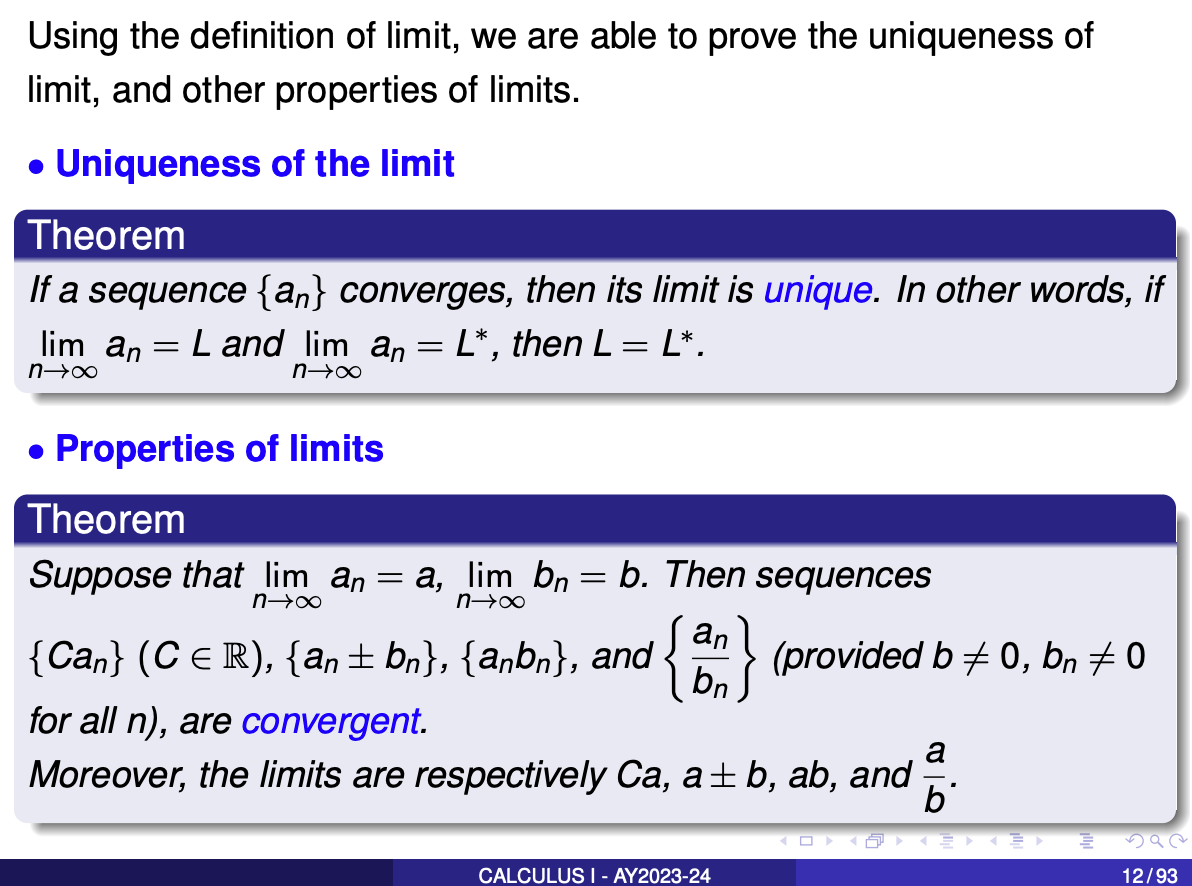
\includegraphics[scale = .55]{Screenshot 2023-12-06 at 3.53.51 PM.png}    

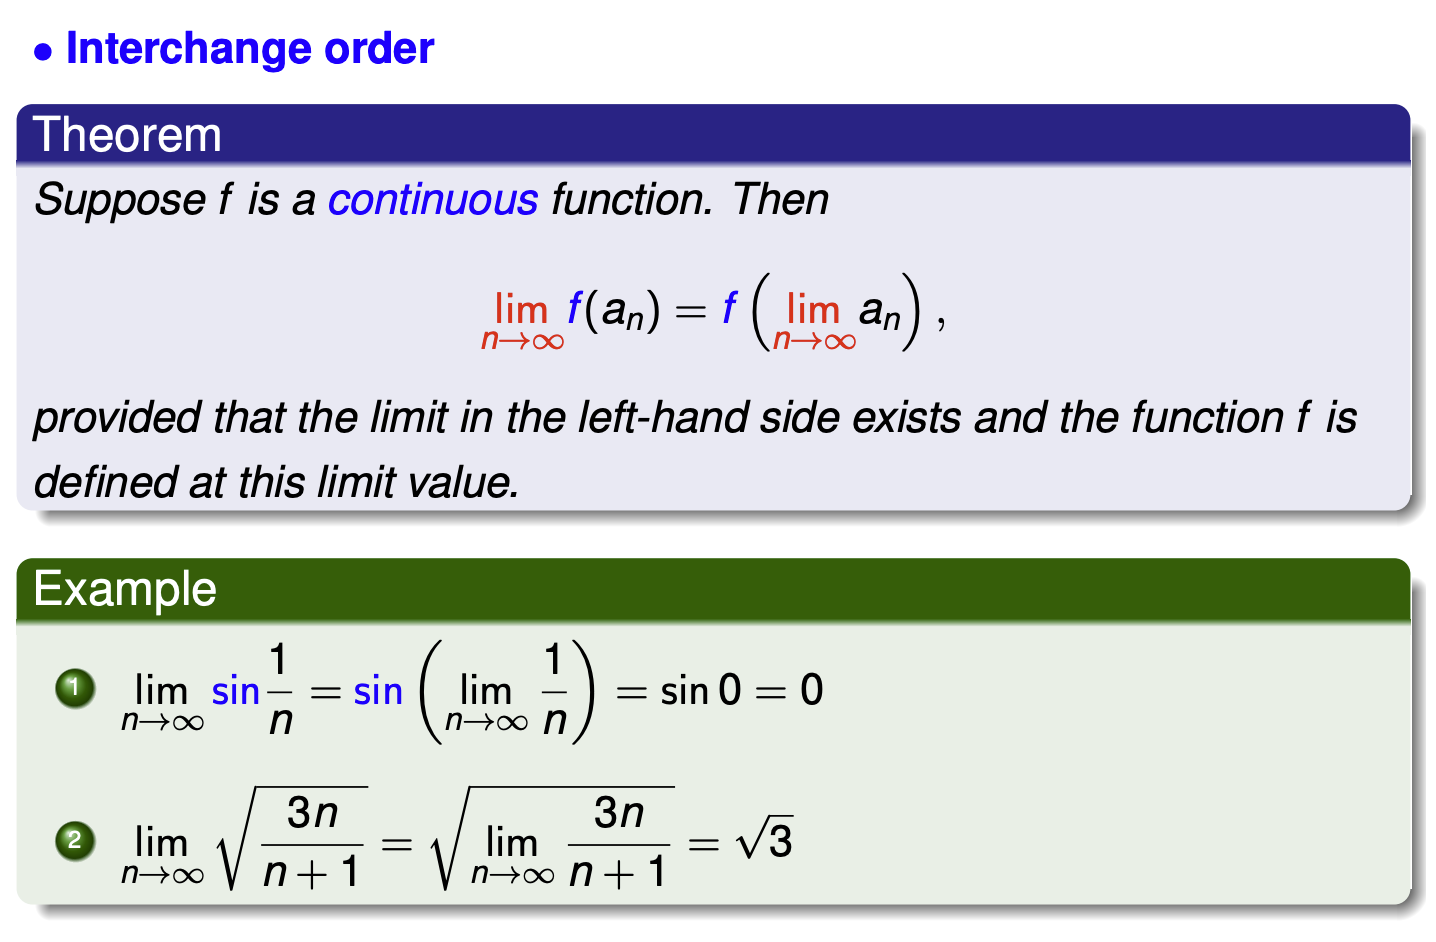
\includegraphics[scale = .45]{Screenshot 2023-12-06 at 3.59.49 PM.png}
\end{center}
For the other limit properties, please review Chapter 1  - Section "Limits".
\subsubsection{Subsequences}
A \textbf{subsequence} of $\left\{a_n \right\}$ is a sequence "extracted" from the sequence $\left\{a_n \right\}$
For examples:
\begin{itemize}
    \item $\left\{a_{n^2} \right\}$, that is $a_1, a_4, a_9, a_{16},...$
    \item The even subsequence $\left\{a_{2n} \right\}$ that is $a_2, a_4, a_6,..., a_{2n}...$
    The odd subsequence $\left\{a_{2n-1} \right\}$ that is $a_1, a_3, a_5,..., a_{2n-1}...$
\end{itemize} A useful property of subsequences is this theorem (Bolzano - Weirstrass Theorem): \textbf{$$ \text{If} \lim_{n\to\infty} a_n = L, \text{then every subsequences of} \left\{a_n \right\} \text{also converges to L.} $$}
\begin{center}
    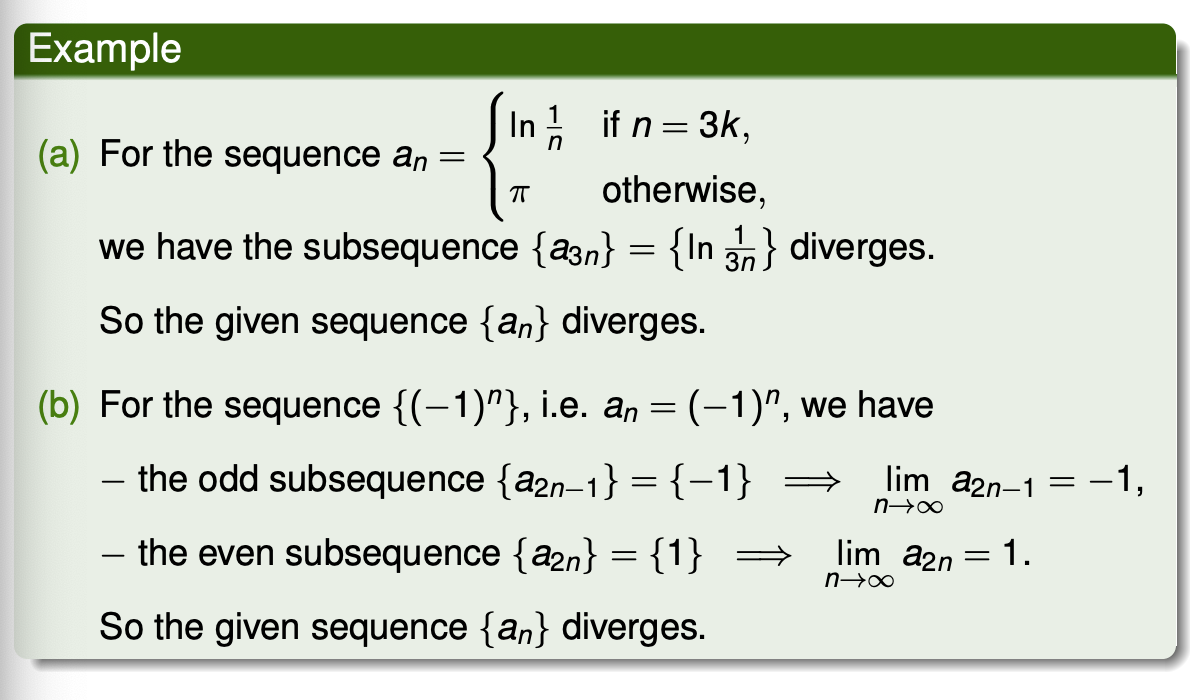
\includegraphics[scale = 0.6] {Screenshot 2023-12-06 at 4.17.38 PM.png}
\end{center}
\subsection{Other properties}
\textbf{Bounded sequence.} A sequence ${a_n}$ is said to be bounded if there are numbers M and m such that: 
$$ m \leq a_n \leq M, \text{ for every n. }$$
Numbers m and M are called a lower bound and an upper bound of the sequence $a_n.$
\begin{mdframed}
If a sequence $a_n$ converges, then it is bounded!
\end{mdframed}
\textbf{Monotone sequences}
\begin{itemize}
    \item A sequence $a_n$ is said to be increasing for $n\geq n_0$ if $a_n \leq a_{n+1} $ for every $n \geq n_0$ (where $n_0$ is some integer).
    \item  A sequence $a_n$ is said to be decreasing for $n\geq n_0$ if $a_n \geq a_{n+1} $ for every $n \geq n_0$ (where $n_0$ is some integer).
    \item A sequence $a_n$ is said to be monotonic if it is either increasing or decreasing. 
\end{itemize}
\begin{mdframed}
Every bounded, monotonic sequence is convergent.
\end{mdframed}




\pagebreak
%
%
%
%
%
%
% PHAN 2: SERIES

\section{Series}
\subsection{Definition}
Let $\left\{a_n \right\}$ be a sequence.  An infinite series is a formal expression (of an “infinite sum”) of the form:
$$\sum_{n=1}^{\infty} = a_1 + a_2 + a_3 + ...$$
To be clear, what makes this as “infinite” sum is the fact that we are adding infinitely many things, NOT that the resulting sum itself might be infinite. Series don’t have to start at 0; for instance:
$$\sum_{n=2}^{\infty} = a_2 + a_3 + a_4 + ...$$
begins the infinite sum at n = 2 instead. In general, the notion says we plug in the first value of n to get the first term, then increase n by 1 to compute the next term, then increase again and so on, adding on each new term we get at each step. 

The key question we care about is whether \textbf{a series converges}, meaning that we actually \textbf{get a finite value} out of the given infinite sum, or \textbf{diverges}, meaning that we \textbf{don’t get a specific value}. \\
\newline
\textbf{Partial Sums}. But to make all of this precise, we have to be more careful about what it actually means for a series to converge. 

Consider the partial sums $s_k$ of the series $\sum_{n=0}^{\infty} $ in question, which are the sums obtained by adding one more term in our series at each step:
\begin{align*}
    s_0 &= a_0 \\
    s_1 &= a_0 + a_1 \\
    s_2 &= a_0 + a_1 + a_2 \\
    &\ \vdots \\
    s_k &= a_0 + a_1 + a_2 + a_3 + ... + a_k = \sum_{n=0}^{k} a_n
\end{align*}
The key point here is that if a series DOES have a finite sum, then as k tends to infinity, the partial sum gets better at approximating the finite value of the series. We arrive at this definition: 
\newline
\begin{mdframed}
The series $\sum_{n=1}^{\infty}$ is said to converge, if the sequence $\left\{s_k \right\}$ converges. Moreover, if  $\lim_{k\to\infty} S_k = S$, then we say the given series \textit{converges} to S, and write $\sum_{n=1}^{\infty}=S$. The number S is called the sum of the series. If a series does not converge, then it is said to \textit{diverge}.
\end{mdframed} 
\textbf{Example 1.} We now investigate whether a series converges or not using the definition: 
$$\sum_{n=1}^{\infty} \frac{1}{n(n+1)}$$
This series is equivalent to: 
$$\sum_{n=1}^{\infty} \left(\frac{1}{n} - \frac{1}{n+1}\right)$$
We can determine the $k^{th}$ partial sum by:
$$S_k = \left(1-\frac{1}{2}\right) + \left(\frac{1}{2} - \frac{1}{3}\right) + \left(\frac{1}{3} - \frac{1}{4}\right) + ... + \left(\frac{1}{k} - \frac{1}{k+1}\right) = 1 - \frac{1}{k+1}$$
It is obvious that: $$\lim_{k\to\infty} S_k = \lim_{k\to\infty} \left(1 - \frac{1}{k+1}\right) = 1 $$
thus, we conclude that the given series converges and its sum is 1.

\subsection{Important series}
Let's have a look at some of the most important series that you have to remember in order to ace the Final Test: 
\begin{enumerate}
    \item Geometric Series:
    $$\sum_{n=0}^{\infty} ar^n = a + ar + ar^2 + ar^3 + ... + ar^n + ...$$
    where $a \neq 0 $ is a constant number, and for any $n>= 0, \frac{a_{n+1}}{a_n} = r$ is also a constant number. (known as the common ratio r)
    \begin{center}
        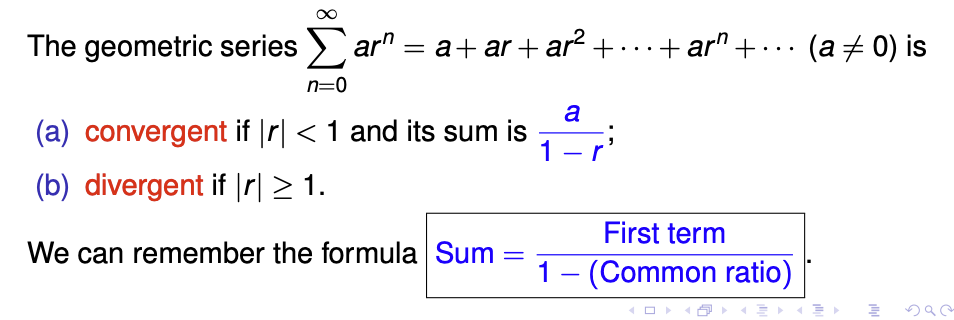
\includegraphics[scale = 0.7]{Screenshot 2023-12-07 at 12.36.24 PM.png}
    \end{center}
    \textbf{Practice 1}: Prove that this series converge and find its sum:
    $$\sum_{n=0}^{\infty} \frac{2 \cdot 3^{n+1}}{5^n}$$ 
    \textbf{Practice 2}: Check whether these series converge or diverge and explain why. If a series converge, find its sum? \\
        \\2a.
        $$\sum_{n=1}^{\infty} (-1)^n \frac{4^{n+2}}{3^{n-1}} \\$$
        \\2b.
        $$\sum_{n=2}^{\infty} \left(\frac{1}{2^n} + \frac{1}{3^n} \right) $$
    \item Harmonic series. Remember that \textbf{this series diverges}:
    \begin{center}
        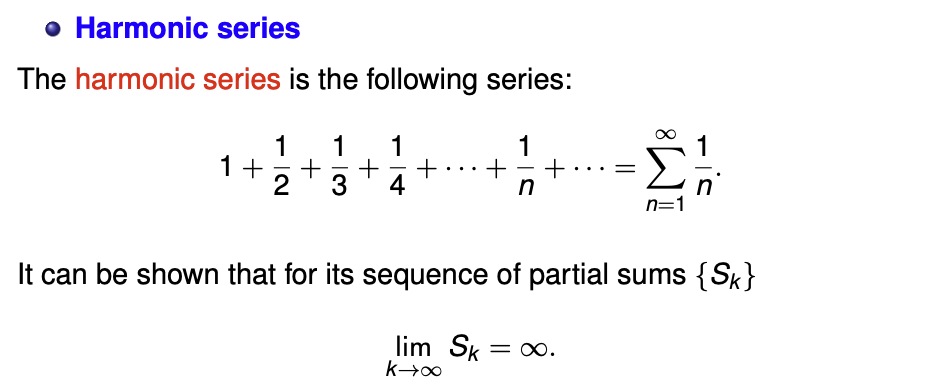
\includegraphics[scale = 0.7]{Screenshot 2023-12-07 at 12.49.12 PM.png}
    \end{center}

    \item Alternating Series. 
     \begin{center}
        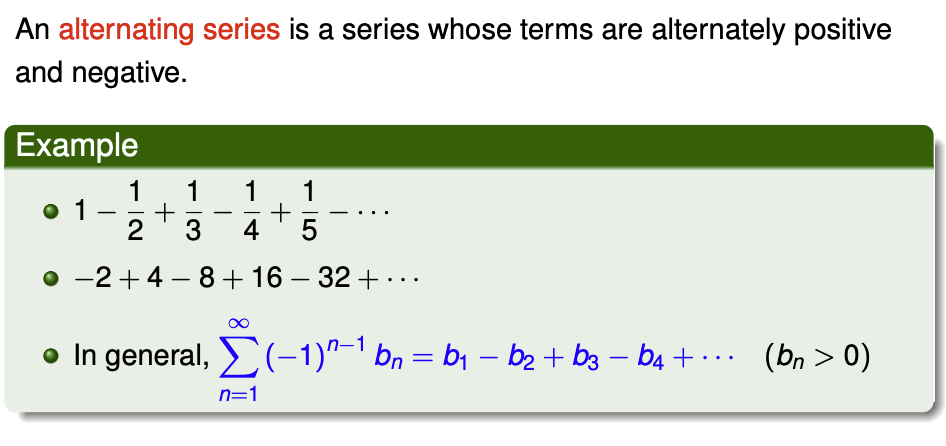
\includegraphics[scale = 0.7]{Screenshot 2023-12-07 at 12.51.51 PM.png}
    \end{center}  

    \item p-series.
    Remember that p-series has this form: 
    $$ \sum_{n=1}^{\infty} \frac{1}{n^{p}}$$
    where p is some constant. It converges when $p > 1$, and diverges if $p \le 1$. We will return to this in the convergence/divergence test part. 
\end{enumerate}

\subsection{Series properties}
Finally, take a look at some basic series properties. 
 \begin{center}
        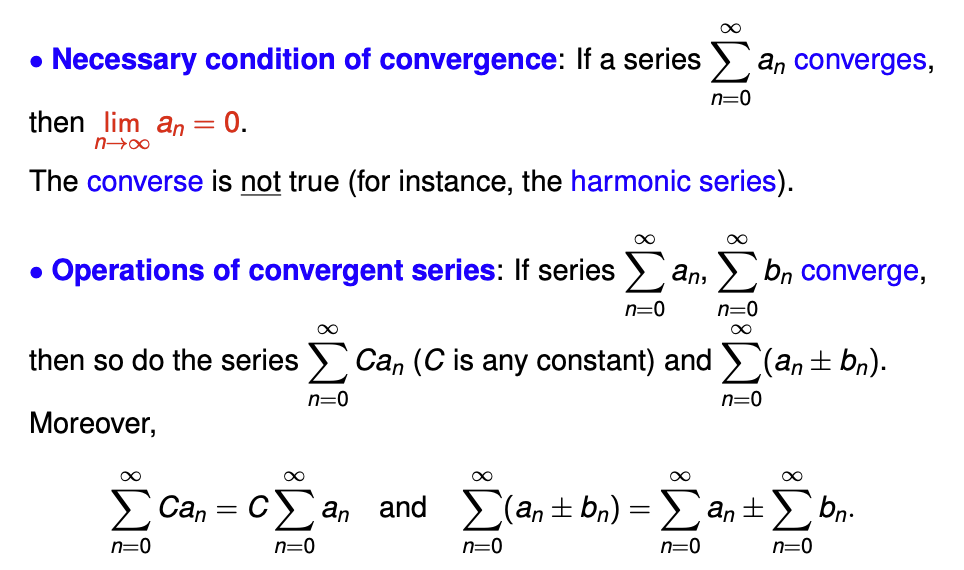
\includegraphics[scale = 0.7]{properties series.png}
    \end{center} 
%Series: Convergence and Divergence Test part 

%
%
%Series Properties
%
%
\section{Series properties}
As I have mentioned before, the key question regarding series is whether \textbf{a series converges}, meaning that we actually \textbf{get a finite value} out of the given infinite sum, or \textbf{diverges}, meaning that we \textbf{don’t get a specific value}. \\
Part 3 would deal with all important types of tests for divergence and convergence. We will also share a strategy for testing this property of a series at the end of this section. This is indeed very important, so please take a close look on this part!
    
\subsection{First Divergence test}
$$\text{In a series} \sum_{n=1}^{\infty} a_n, \text{if the sequence } a_n \text{ does not converge to } 0, \text{the series}  \sum_{n=1}^{\infty} a_n \text{ must diverge.}$$
\\
\textbf{Example:} Consider the series: 
$$ \sum_{n=1}^{\infty} n^{1/n}$$
First and foremost, we should use the n-th term test (Or, in this document, First Divergence Test):
$$ \lim_{n\to\infty} n^{1/n} $$
The limit leads to the indeterminate form $(\infty)^0. $ We let $ f(n) = n ^ {1/n}$ and find $\lim_{n\to\infty} \ln{f(n)}. $ Since:
$$ \ln{f(n)} = \ln{n^{1/n}} = \frac{\ln{n}}{n}$$
Applying the l'Hôpital rule gives: 
   $$ \lim_{n\to\infty} \ln{f(n)} = \lim_{n\to\infty} \frac{\ln{n}}{n} 
    = \lim_{n\to\infty} \frac{1/n}{n} = 0$$
Therefore, 
$$ \lim_{n\to\infty} n^{1/n} = \lim_{n\to\infty} f(n) =  \lim_{n\to\infty} e^{\ln{f(n)}} = e^0 = 1 $$
As the n-th term test shows that the sequence converges to 1, which is different from 0, we conclude that the series diverges. 

 \subsection{Geometric Series test}
Recall that a geometric series has the form: 
 $$\sum_{n=0}^{\infty} ar^n = a + ar + ar^2 + ar^3 + ... + ar^n + ...$$
where $a \neq 0 $ is a constant number, and for any $n>= 0, \frac{a_{n+1}}{a_n} = r$ is also a constant number. (known as the common ratio r). \\
It is easy to determine whether a geometric series converges or diverges: return to the geometric series introduction in section 2.2 to check this. 

\subsection{Study of non-negative series}
These are series with non-negative terms: 
$$ \sum_{n=1}^{\infty} a_n, a_n \leq 0 \text{ for all } n.$$
There are special techniques for testing the convergence of these series. \\
 \begin{center}
        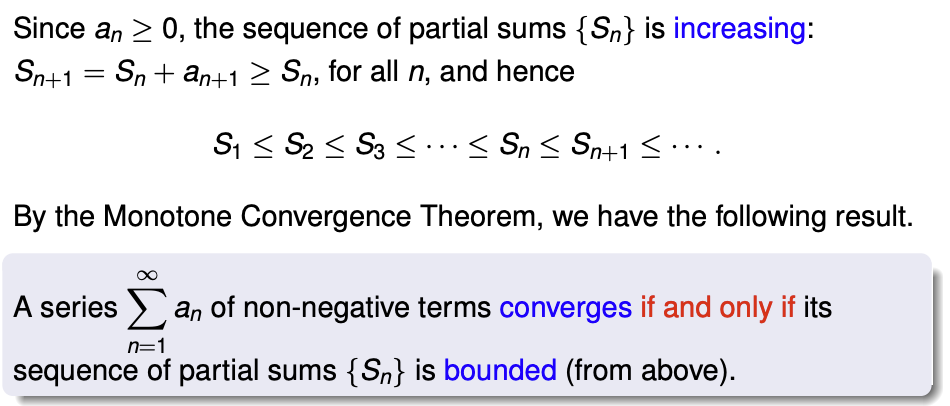
\includegraphics[scale = 0.7]{non-negative series.png}
    \end{center} 

\subsubsection{Integral Test}
The integral test applies to series of the form:
$$ \sum_{n=1}^{\infty} f(n)$$
where $f$ is a continuous, positive, \textit{decreasing} function \\
In this setting, the series $ \sum_{n=1}^{\infty} f(n)$ and the improper integral $\int_1^{\infty} f(x) dx$ both behave in the same way, meaning they both converge or they both diverge. Therefore, we can turn problems about series convergence into ones about integral convergence instead. \\ \\ 
\textbf{IMPORTANT. }Remember to state that $f(n)$ satisfies all the condition before doing the integral test so that you would not lose 0.25 - 0.5pt in the test! \\ \\
\textbf{Example 1.} Consider the harmonic series: 
$$ \sum_{n=1}^{\infty} \frac{1}{n} $$
This function satisfies the three conditions to apply the integral test: Continuous, Positive, and Decreasing. This means that we can now apply the integral test. Consider the integral:
$$ \int_{1}^{\infty} \frac{1}{x} dx$$
We get:
$$ \int_{1}^{\infty} \frac{1}{x} \, dx = \lim_{b \to \infty} \int_{1}^{b} \frac{1}{x} \, dx = \lim_{b \to \infty} \ln x \Big|_{1}^{b} = \lim_{b \to \infty} (\ln b - 1) = \infty.$$
We conclude this series diverges. \\ \\
\textbf{Example 2.} Consider the series: 
$$ \sum_{n=2}^{\infty} n^2 e^{-n^3}$$
Observe: 
\begin{itemize}
    \item This series starts with $n=2$. We should consider the integral from 2, not 1 like the previous example.
    \item We can prove that we can use the integral test, as this satisfies the three necessary conditions (Prove it!)
\end{itemize}

Now we start doing the integral test: 
\begin{align*}
    \int_{2}^{\infty} x^{2} e^{-x^{3}} dx = \lim_{b\to\infty} \int_{2}^{b} x^{2} e^{-x^{3}} dx 
&= \lim_{b\to\infty} \left( -\frac{1}{3} e^{-x^{3}} \right) \Big|_{2}^{b} \\
&= \lim_{b \to \infty} \left( -\frac{1}{3} \left( e^{-b^{3}} - e^{-8} \right) \right) \\
&= -\frac{1}{3} e^{-8} .
\end{align*}

This integral converges, so the integral test says that the given series also converges! \\ \\
\textit{Using the integral test, determine whether these series converge or diverge} 
\begin{enumerate}
    \item $$ \sum_{n=3}^{\infty} \frac{n^2}{n^3 + 1}$$
    \item $$ \sum_{n=2}^{\infty} \frac{1}{n \ln{n}}$$
\end{enumerate}

\subsubsection{p-series test.}
Remember that p-series has this form: 
    $$ \sum_{n=1}^{\infty} \frac{1}{n^{p}}$$
    where p is some constant. It converges when $p > 1$, and diverges if $p \le 1$.


\subsubsection{Direct comparison test.} 
The key facts to remember are: 
\begin{itemize}
    \item If the larger series converges, so does the smaller one.
    \item If the smaller series diverges, so does the larger one. 
    \item We must "guess" the proper series to do this - therefore, this is a hard method. 
\end{itemize} 
\textbf{Example 1.} Consider the series: 
$$ \sum_{n=1}^{\infty} \frac{10n^2 - 3n -1}{n^4 + n^2 + 1}$$
Observe that: 
$$ 0 \leq \sum_{n=1}^{\infty} \frac{10n^2 - 3n -1}{n^4 + n^2 + 1} \leq \frac{10n^2}{n^4} = \frac{10}{n^2} $$
Sine the sum on the right and the left are all finite, the infinite sum should be finite. We conclude the given series converges by the direct comparison test. \\
\textbf{Example 2. } Consider the series: 
$$ \sum_{n=1}^{\infty} \frac{cos^2(n)}{n^{3/2}}$$
Observe that:
$$ \sum_{n=1}^{\infty} \frac{cos^2(n)}{n^{3/2}} \leq \sum_{n=1}^{\infty} \frac{1}{n^{3/2}}   (\text{As } 0 \leq cos^2(n) \leq 1)$$
By the p-series test, $\sum_{n=1}^{\infty} \frac{1}{n^{3/2}}$ converges. 
Therefore: $ \sum_{n=1}^{\infty} \frac{cos^2(n)}{n^{3/2}}$ converges


\subsubsection{Limit comparison test.} 
This test only applies to series consisting of positive terms. For such series $ \sum a_n$ and $\sum b_n$, look at the limit: 
$$ L = \lim_{n\to\infty} \frac{a_n}{b_n}$$
If L exists and is positive, series $ \sum a_n$ and $\sum b_n$ behaves in the same way: Both will converge or diverge. \\
\textbf{Example.} Consider the series: 
$$\sum_{n=5}^{\infty} \frac{n(1-e^{-n})}{n^3 + 3}$$
Focusing on dominant terms only suggests that this series should behave like: 
$$ \sum_{n=5}^{\infty} \frac{n}{n^3} = \sum_{n=5}^{\infty} \frac{1}{n^2}$$
We use the limit comparison test. Look at the limit: 
$$\lim_{n\to\infty} \frac{\frac{n(1-e^{-n})}{n^3 + 3}}{\frac{1}{n^2}}$$
We can prove that the limit is 1. As the limit is \textit{finite and positive}, since $\sum \frac{1}{n^2}$ converges, our given series does converge! \\
\textbf{Warning.} When limit $L = 0$, we can't determine whether the two series behave in the same way or not. 

\subsection{Ratio Test, Root Test and Absolute Convergence}
\subsubsection{Ratio Test and Root Test}
\begin{center}
        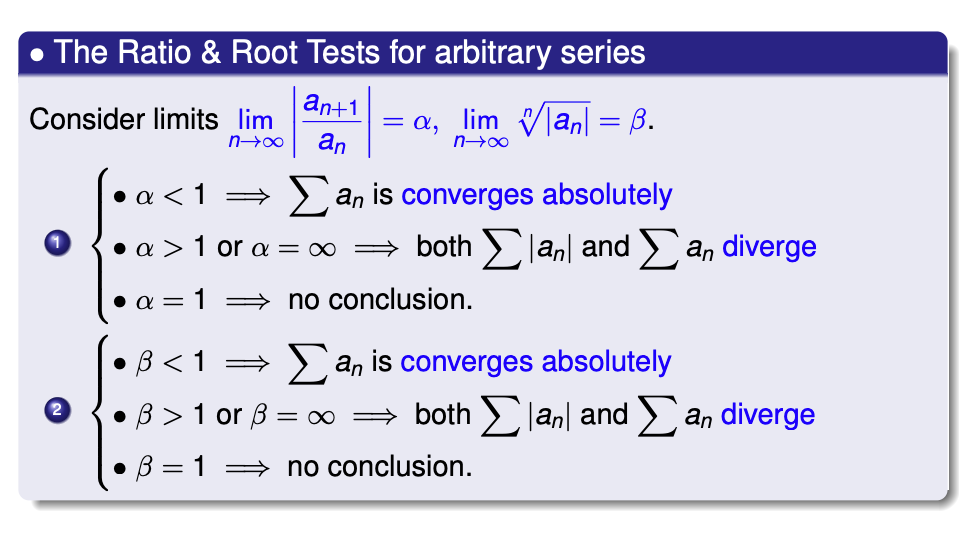
\includegraphics[scale = 0.7]{ratio - root test.png}
    \end{center} 
We take a look at some examples: \\ \\
\textbf{Example 1.} Consider the series: 
$$\sum_{n=1}^{\infty} (-1)^n \frac{n}{5^n}$$
In the notation of the ratio test, $a_n = (-1)^n \frac{n}{5^n}$, so we compute the limit: 
$$\lim_{n \to \infty} \frac{|a_{n+1}|}{|a_n|} = \lim_{n \to \infty} \frac{\left| (-1)^{n+1} \frac{ n+1}{5^{n+1}}\right|}{\left|(-1)^n \frac{n}{5^n}\right|} = \lim_{n \to \infty} \frac{(n + 1)5^n}{n5^{n+1}} = \lim_{n \to \infty} \frac{n + 1}{5n} = \frac{1}{5}.$$
Since this limit is less than 1, the ratio test tells us that this series converges
\\ \\
\textbf{Example 2.} Consider the series: 
$$\sum_{n=0}^{\infty} \frac{(-3)^n}{(2n+1)!}$$
We compute the following limit:
$$\lim_{n \to \infty} \frac{\left| \frac{(-3)^{n+1}}{(2(n+1)+1)!} \right|}{\frac{(-3)^n}{(2n+1)!}} = \lim_{n \to \infty} \frac{3^{n+1}}{(2n + 3)!} \frac{(2n+1)!}{3^n} = \lim_{n \to \infty} \frac{3}{(2n + 3)(2n + 2)} = 0.$$
Since we got a limit of zero, the ratio test implies that our given series converges. \\ \\
\textbf{Example 3.} Consider the series:
$$ \sum_{n=1}^{\infty} (-1)^n \left(1-\frac{1}{n}\right)^{n^2}$$
We do the root test: 
   $$ \lim_{n\to\infty} \sqrt[n]{\left|(-1)^n \left(1-\frac{1}{n} \right)^{n^2} \right|}  = \lim_{n\to\infty} \left(1-\frac{1}{n}\right)^n$$
Note that $e^x = (1 + \frac{x}{n})^n$. Therefore:
$$ \lim_{n\to\infty} \left(1-\frac{1}{n}\right)^n = \frac{1}{e} < 1$$
According to the root test, this series converges absolutely. 


\subsubsection{Absolute Convergence}
 \begin{center}
        \includegraphics[scale = 0.7]{def: absolute convergence.png}
    \end{center} 
 \begin{center}
        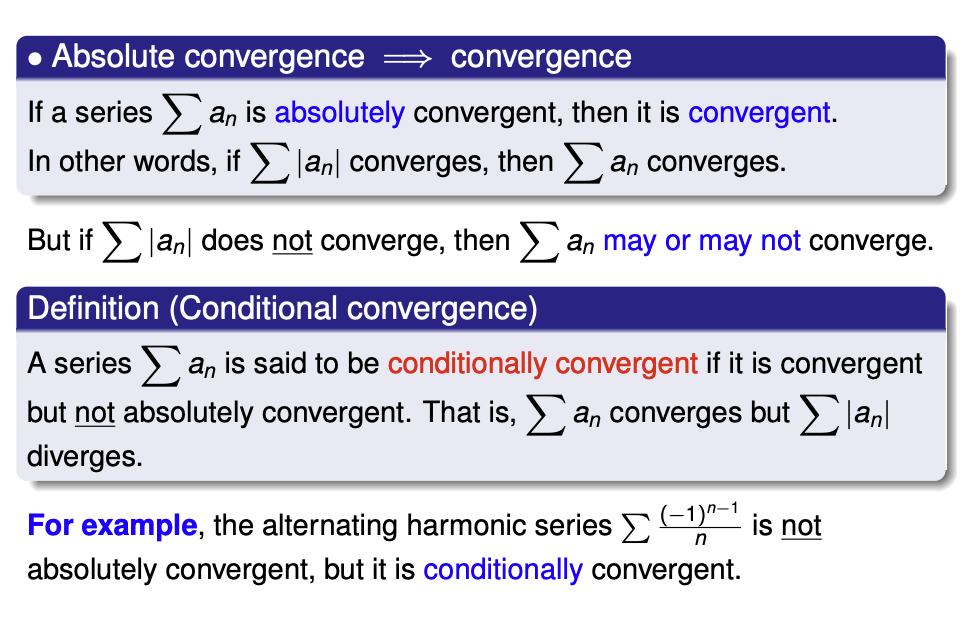
\includegraphics[scale = 0.7]{conditional convergence.png}
    \end{center} 
\textbf{Why investigate absolute and conditional convergence?} For the sake of brevity, I will not include this in this document. However, you can find an explanation in the appendix of this document, or read the books if you are curious enough! 
\subsection{Alternating Series Tests}
 \begin{center}
        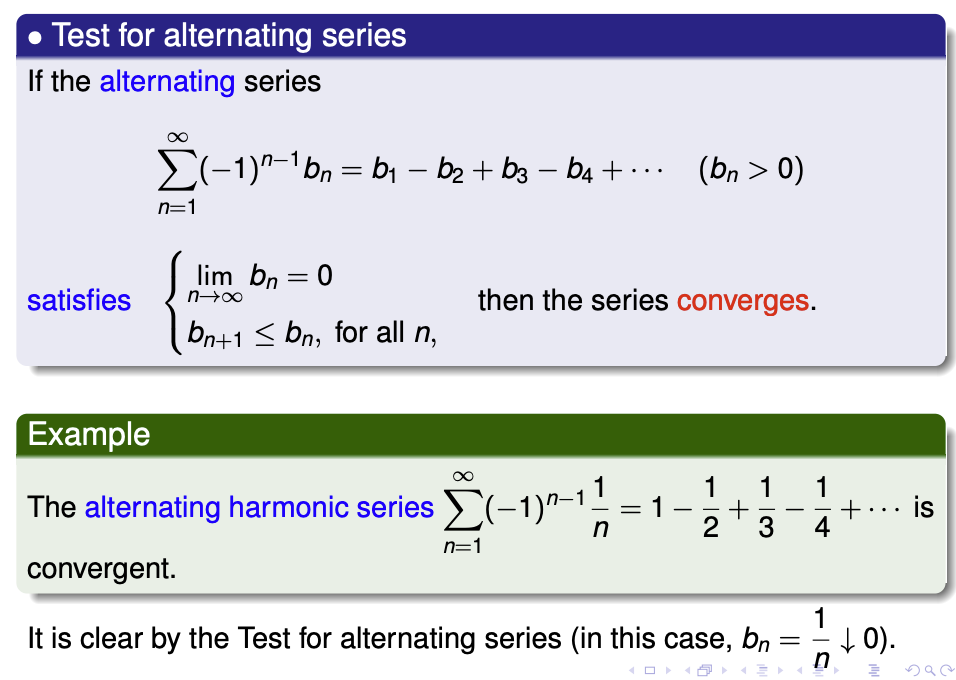
\includegraphics[scale = 0.7]{Screenshot 2023-12-07 at 1.06.23 PM.png}
    \end{center} 
\textbf{IMPORTANT.}Remember to state that $b_{n+1} \leq b_n$ in your exam so that you would not lose 0.25pt in the test.  

\subsection{Convergence Strategies}
\begin{itemize}
    \item Use first and foremost the n-th term test.
    \item If the given series has the form of geometric or p-series, use the corresponding test for them.  This applies to alternating series test too. 
    \item If not possible, try ratio/root test next. This is highly effective for series with factorials!
    \item Try limit comparison test next if nothing has worked so far. This works especially with fractions whose numerator and denominators (tử số và mẫu số) only involve powers of n. 
    \item Integral test may be used, but remember to check all the necessary conditions: positive, continuous and decreasing function. 
    \item Direct comparison test might be the toughest one. However, for any series with involves sine or cosine, perhaps this is the first test you should use, as sine and cosine terms are usually simple to bound. 
\end{itemize}

\textbf{Exercise: Determine whether these series converges or diverges?}
\begin{align*}
&1. \sum_{n=1}^{\infty} \frac{2^n}{3^n} && 2. \sum_{n=1}^{\infty} \frac{1}{n^2 + 30} && 3. \sum_{n=1}^{\infty} \frac{1}{2\sqrt{n}+ \sqrt[3]{n}} \\
&4. \sum_{n=1}^{\infty} \frac{\sin^2{n}}{2^n} && 5. \sum_{n=1}^{\infty} \frac{2n}{3n-1} && 6. \sum_{n=3}^{\infty} \frac{1}{\ln{(\ln{n})}} \\
&7. \sum_{n=1}^{\infty} \frac{3^n}{n!} && 8. \sum_{n=1}^{\infty} \left(\frac{3n+1}{2n} \right)^n && 9. \sum_{n=1}^{\infty} \frac{\sqrt{n^3 + n}}{n^4 - n^2}
\end{align*}
\\
\\
%Taylor series (TAYLOR SWFIT I LOVE U)

%
%
%%Section: Power Series
%
%
\section{Power Series. Taylor and Maclaurin Series}
\subsection{Power Series}
$$\frac{1}{1-x} = \sum_{n=0}^{\infty}x^n \text{ where } |x| < 1$$
Now, we view the right side as a \textit{function} by treating $x$ as a variable: plugging in a value of $x$ into this series gives the value on the left side. We can say that the series $\sum_{n=0}^{\infty}x^n$ represents the function $\frac{1}{1-x}$ on the interval (-1, 1). Representing functions as series is the whole reason why we care about series in the first case! \\
\begin{center}
        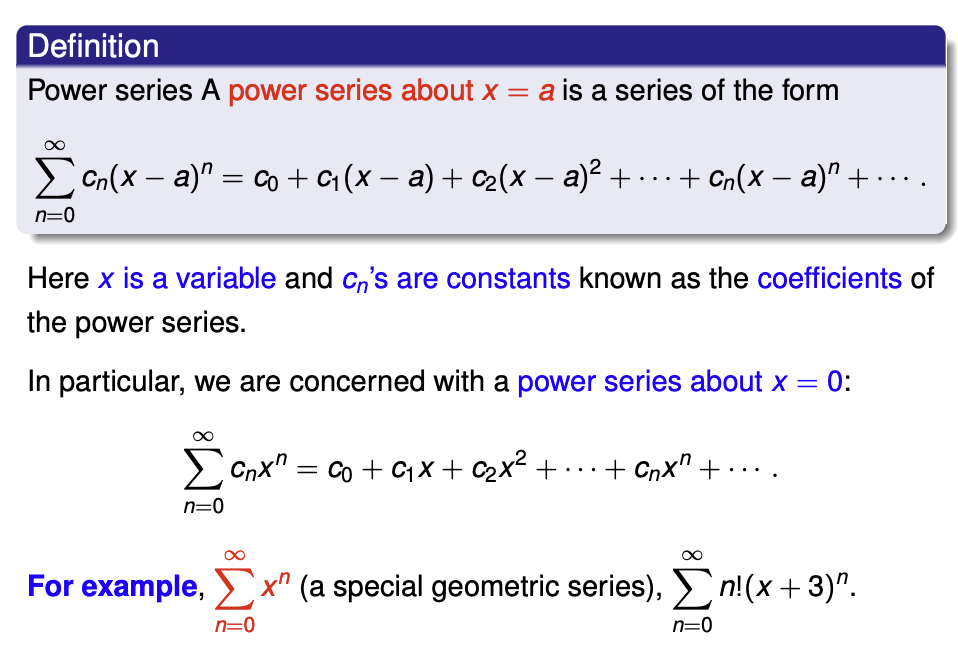
\includegraphics[scale = 0.7]{power series - def.png}
    \end{center} 
\textbf{Example 1.} The power series: 
$$ \sum_{n=0}^{\infty} (3x-1)^n$$
As we have: 
$$ \frac{1}{1-y} = \sum_{n=0}^{\infty} y^n$$ Let $y=3x-1$:
$$\frac{1}{1-(3x-1)} = \sum_{n=0}^{\infty} (3x-1)^n$$
This series will converge when $|y| < 1$, so when: 
$$ |3x - 1| < 1 \Leftrightarrow 
\left|x - \frac{1}{3} \right| < \frac{1}{3} \Leftrightarrow 0 < x < \frac{2}{3}$$
We conclude that the given series converges for $ x \text{ in }\left(0, \frac{2}{3}\right)$, thus: 
$$ \frac{1}{2-3x} = \sum_{n=0}^{\infty} (3x - 1)^n = \sum_{n=0}^{\infty} 3^n \left(x-\frac{1}{3} \right)^n $$
represents the function $\frac{1}{2-3x}$ as a power series centered at $\frac{1}{3} \text{ on the interval} \left(0, \frac{2}{3}\right)$

\subsection{Interval of Convergence}
We test a power series for convergence by using various tests to see where it converges and diverges. For the geometric series, for example, it diverges when $|r| > 1$, and converges when $ |r| < 1.$ How about for other series? \\
One key fact is that any \textbf{power series} converges for $x$ in some \textit{interval} around its center a. There are three possible cases: 
\begin{itemize}
    \item Converges absolutely for all x
    \item Converges at only one point x = a 
    \item Converges when $|x-a| < R$ and diverge when $|x-a| > R$, with R is a \textbf{positive real number.}
\end{itemize}
We now get to some definitions: 
\begin{center}
        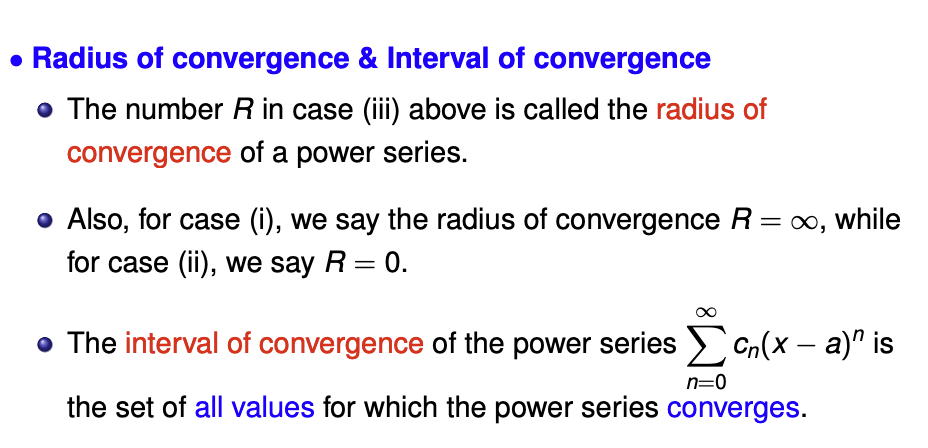
\includegraphics[scale = 0.7]{radi convergence.png}
        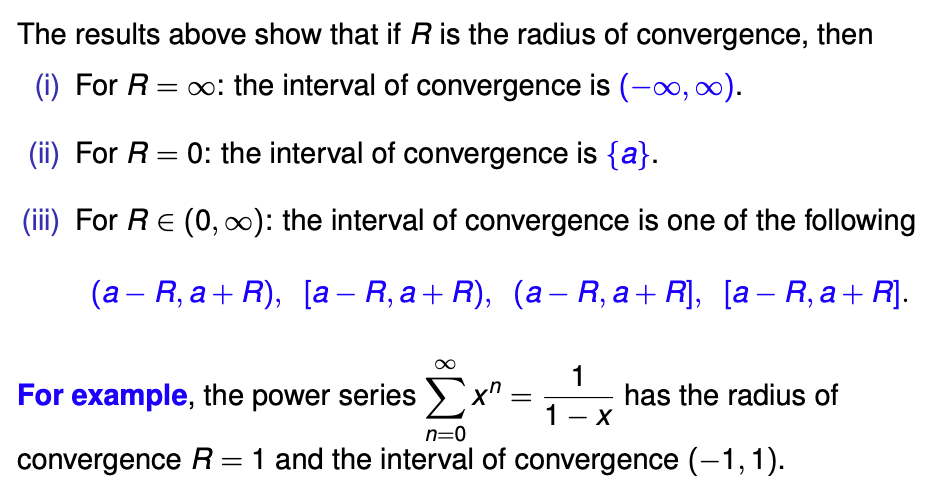
\includegraphics[scale = 0.7]{implications of radius .png}
    \end{center} 
Find the interval and radius of convergence is an application of the ratio test! It is on this interval that we can make sense of saying that the power series in question represents a function, since this interval characterizes the values of x we can actually plug into that function and have the resulting value make sense. \\ \\ 
\textbf{Example 1. }Find the interval of convergence of this series: 
 $$ \sum_{n=1}^{\infty} n(x-2)^n$$
    Using the ratio test: 
    $$\lim_{n \to \infty} \frac{|a_{n+1}|}{|a_n|} = \lim_{n \to \infty} \frac{(n + 1)|x - 2|^{n+1}}{n|x - 2|^n} = \lim_{n \to \infty} \frac{(n + 1)|x - 2|}{n} = |x - 2| \lim_{n \to \infty} \left( 1 + \frac{1}{n} \right) = |x - 2|. $$
According to the ratio test, the given series converges when $|x-2| <  1$, and diverges when $|x-2| >1$. In other words, the series converges at least for $x \in (1,3).$ 

Recall that the ratio test is inconclusive when $\lim_{n\to\infty} \frac{|a_{n+1}|}{|a_n|} = 1.$ We must test the case when $x=1 \text{ and when } x = 3.$ Testing gives us that when $x=1 \text{ or } x=3$, our series diverges. Only after this step can we conclude the interval of convergence is (1,3). \\ \\ 
\textbf{Example 2. }Find the interval of convergence of this series: 
$$\sum_{n=0}^{\infty} (2n+1)!(x-1)^n$$
    Using the ratio test: 
    $$ \lim_{n\to\infty} \frac{(2(n+1)+1)! |x-1|^{n+1}}{(2n+1)!|x-1|^n} = \lim_{n\to\infty} \frac{(2n+3)!}{(2n+1)!} |x-1|= \lim_{n\to\infty} (2n+3)(2n+2)|x-1| $$
    We can see that $(2n+3)(2n+2)$ goes to infinity for any $x$ except $x=1$. This is less than 1, so the ratio test tells us that the given series does converge when $x=1. $  \\
    Conclusion: The series converges only when $x=1$, and thus the interval of convergence consists of just the single point 1. \\ \\
\textbf{Example 3. }Find the interval of convergence of this series:
$$ \sum_{n=0}^{\infty} \frac{x^n}{n!}$$
Using the ratio test:
$$ \lim_{n\to\infty} \frac{|x|^{n+1}}{(n+1)!|x|^n} = \lim_{n\to\infty} \frac{|x|}{n+1} = 0$$
This is smaller than 1 no matter what x is, we conclude that series: 
$$ \sum_{n=0}^{\infty} \frac{x^n}{n!}$$
does converges for all x. The interval of convergence is thus $(-\infty, \infty)$, and we say that the radius of convergence is $\infty$. In this case there are no endpoints to check! 

\subsection{Series Manipulation}
\subsubsection{Subtitution}
From the basic power series: 
$$ \frac{1}{1-y} = \sum_{n=0}^{\infty} y^n$$ 
we can substitute $ y = f(x) $ on both sides. This is what we call Substitution. \\ \\ 
\textbf{Example 1.} What function does this series represent?
$$ \sum_{n=0}^{\infty} (-1)^n x^{2n}$$
From the basic power series, setting $ y = -x^2$ gives: 
$$ \sum_{n=0}^{\infty} (-x^2)^n =  \sum_{n=0}^{\infty} (-1)^n x^{2n}$$
which is precisely the series we're asking about. We thus get: 
$$ \frac{1}{1-(-x^2)} =  \frac{1}{1+x^2} = \\sum_{n=0}^{\infty} (-1)^n x^{2n}$$
This is valid on the interval (-1, 1). 

\subsubsection{Differentiation}
You can differentiate both sides of the basic power series to get some new series. This process is called term-by-term differentiation, and is represented by: 
\begin{center}
        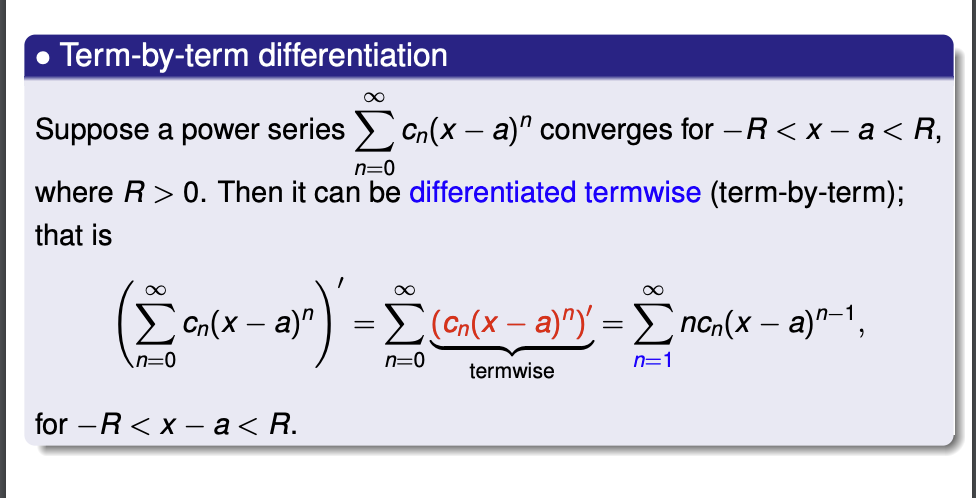
\includegraphics[scale = 0.7]{differentiation.png}
\end{center}
\textbf{Example 1. } Differentiate the standard geometric series: 
$$ \frac{1}{1-x} = \sum_{n=0}^{\infty} x^n$$
Solution: 
\begin{align*}
     \frac{\mathrm{d} }{\mathrm{d} x} \left(\frac{1}{1-x}\right) &=  \frac{\mathrm{d} }{\mathrm{d} x} \left(\sum_{n=0}^{\infty} x^n \right) \\
     \frac{1}{(1-x)^2} &=\sum_{n=0}^{\infty} \frac{\mathrm{d} }{\mathrm{d} x} x^n \\
     &= \sum_{n=1}^{\infty} nx^{n-1} \\
     &= \sum_{n=1}^{\infty} nx^n\frac{1}{x}
\end{align*}
To be clear, we start the final series at $n=1$ since the $n=0$ term is zero anyway, so it is not worth writing. Multiplying through by $x$ would then give the following series representation: 
$$ \frac{x}{(1-x)^2} = \sum_{n=1}^{\infty} nx^n$$
\textbf{Example 2.} Consider the series: 
$$ \sum_{n=1}^{\infty} (-1)^n 2nx^{2n-1}$$
The key observation here is that: 
$$ \left(\sum_{n=0}^{\infty} (-1)^n x^{2n} \right)' = \sum_{n=1}^{\infty} (-1)^n2nx^{2n-1}$$
Since:
$$ \frac{1}{1+x^2} = \sum_{n=0}^{\infty} (-1)^n x^{2n}$$
the series we're looking at in this example should represent the function obtained  by differentiating the left-hand side. By doing this: 
\begin{align*}
    \frac{-2x}{(1+x^2)^2} &= \sum_{n=1}^{\infty} (-1)^n2nx^{2n-1} \\ 
    \text{or }-\frac{x}{(1+x^2)^2} &=  \sum_{n=1}^{\infty} (-1)^nnx^{2n-1}
\end{align*}
\textit{Exercise: Which function is represented by this series: }
$$ \sum_{n=2}^{\infty} n(n-1)x^n$$

\subsubsection{Integration}
Similarly, integrating both sides of the series is valid, and a summary for this process is here:
\begin{center}
        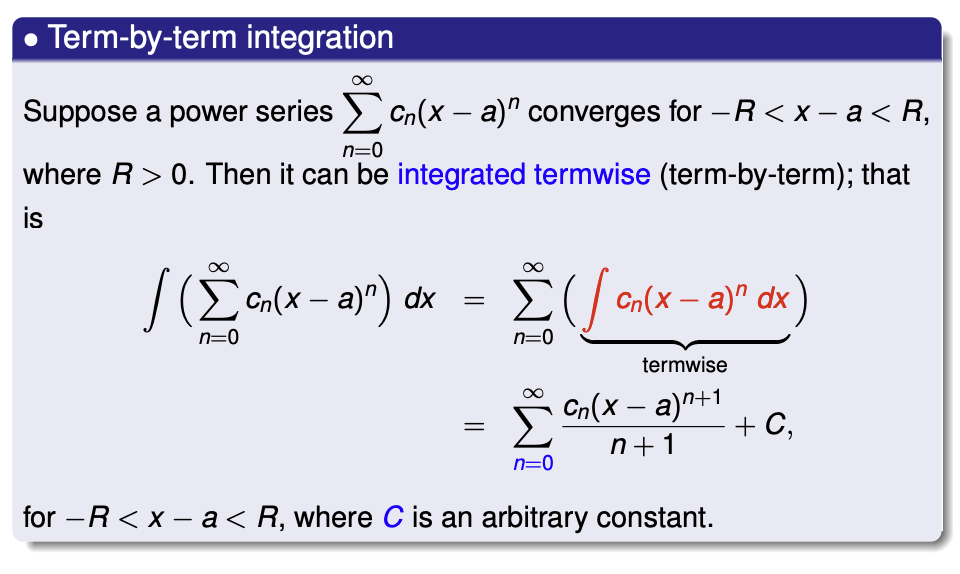
\includegraphics[scale = 0.65]{integration.png}
\end{center}
You can take a look at this example: 
\begin{center}
        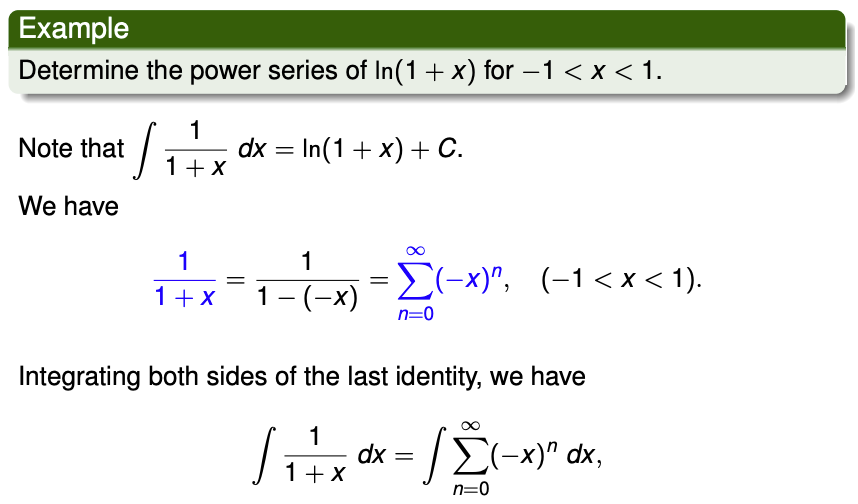
\includegraphics[scale = 0.65]{p1-integration-ex.png}
        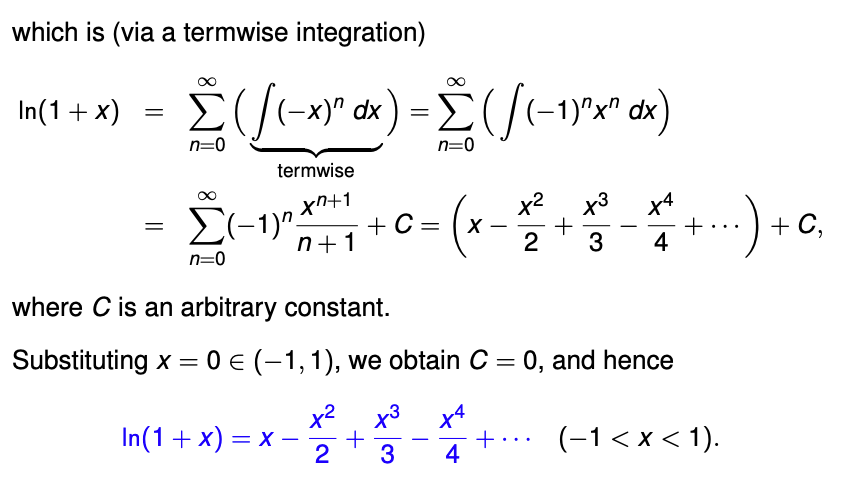
\includegraphics[scale = 0.65]{p2-integration-ex.png}
\end{center}
\subsection{Taylor and Maclaurin Series}
\textbf{Definition.} If we want to express $f$ as a power series centered at a: 
$$ f(x) = \sum_{n=0}^{\infty} c_n (x-a)^n,$$
the coefficients needed must be given by $c_n = \frac{f^{(n)}(a)}{n!}$. The resulting power series: 
$$ \sum_{n=0}^{\infty} \frac{f^{(n)}(a)}{n!} (x-a)^n$$
is called the \textit{\textbf{Taylor series} of f centered at a} and is the only power series which could possibly equal the function $f(x)$ on its interval of convergence. Taylor series which are centered at 0 will be called \textit{\textbf{Maclaurin series}}
$$ \sum_{n=0}^{\infty} \frac{f^{(n)}(0)}{n!}x^n$$
\\ 
\\
There are several important things you should learn by heart: 
\begin{itemize}
    \item In general, the Taylor series generated by a function may or may not be $f(x)$.
    \item However, the theorem (about power series representation) says that if $f$ is representable as a power series at $a$, then the power series is ít Taylor series.
    \item Many functions have power series representation, e.g, $\frac{1}{1+x}, \ln{(1+x)}, e^x, sin x, (1+x)^{\alpha}$
    \item However, there exist functions that are differentiable but has no power series representation!
\end{itemize}

\textbf{Taylor polynomials.} The Taylor polynomial of degree n of $f$, denoted by $T_n(x),$ is defined as follows:
$$ T_n(x) = f(a) + \frac{f'(a)}{1!}(x-a) + \frac{f''(a)}{2!}(x-a)^2 + ... \\
+ \frac{f^{(k)}(a)}{k!}(x-a)^k + .... + \frac{f^{(n)}(a)}{n!}(x-a)^n$$

The coefficient of $(x-a)^k $  is:
$$ c_k = \frac{f^{(k)}(a)}{k!} (k = 0, 1, 2, ..., n)$$  

\newpage
\textbf{Example 1.} Find the Taylor series and the Taylor polynomials generated by $f(x) = e^x $ at $ x = 0$ 
$$ f^{(n)}(x) = e^x \text{ and } f^{(n)}(0) = 1 \text{ for every } n = 0, 1, 2...$$
Therefore, the Taylor series generated by $f$ at $x=0$ is:
\begin{align*}
    f(0) + f'(0)x + \frac{f''(0)}{2!}x^2 + ... + \frac{f^{(n)}(0)}{n!}x^n + .... \\
    &= 1 + x + \frac{x^2 }{2} + ... + \frac{x^n}{n} \\
    &= \sum_{k=0}^{\infty} \frac{x^k}{k!}
\end{align*}
The Taylor polynomial of order n at $x=0$ is:
$$ P_n(x) = 1 + x + \frac{x^2}{2} + ... + \frac{x^n}{n!}$$
\newline
\textbf{Example 2. } Find the Taylor series and Taylor polynomials generated by $f(x) = cos x $ at $ x= 0$ \\ 
\textit{Solution. } The cosine and its derivatives are: 
\begin{align*}
    f(x) &= cos x & f'(x) &= -sin x \\
    f''(x) &= -cos x & f^{(3)}(x) &= sin x \\
    & \vdots &  &\vdots \\
    f^{(2n)}(x) &= (-1)^n cosx & f^{(2n+1)}(x) &= (-1)^{n+1} sinx
\end{align*}
The Taylor series generated by $f$ at 0 is: 
\begin{align*}
    f(0) + f'(0)x &+ \frac{f''(0)}{2!}x^2 + ... + \frac{f^{(n)}(0)}{n!}x^n + ... \\
    &= 1 + 0.x  - \frac{x^2}{2!} + 0\cdot x^3 + \frac{x^4}{4!} + ... + (-1)^n \frac{x^{2n}}{(2n)!} +... \\
    &= \sum_{k=0}^{\infty} \frac{(-1)^kx^{2k}}{(2k)!}
\end{align*}

\textbf{Taylor remainder.} Suppose a function $f$ has derivatives of all orders in an open interval $l$ containing $a$. Then for each $x \in I $ and each positive integer $n$, we have: 
$$ f(x) - T_n(x) = \frac{f^{(n+1)}(c)}{(n+1)!}(x-a)^{n+1}$$
where c is some value between a and x. \\
The expression: 
$$ R_n = \frac{f^{(n+1)}(c)}{(n+1)!}(x-a)^{n+1}$$ is called the Taylor remainder of order n or the error term for the approximation of $f $ by $T_n(x).$

\subsection{Applications of Taylor Series}
This section contains difficult exercise - According to Prof. Khoi Le Hai, these exercises are very difficult, and should you see them appearing in your exam, consider leaving them until you have done the other problems. Therefore, if you aim to just "pass" the subject, I highly recommend not reading this section and revising the previous parts of this sequences - series. 
\subsubsection{Convergence} 
\begin{center}
    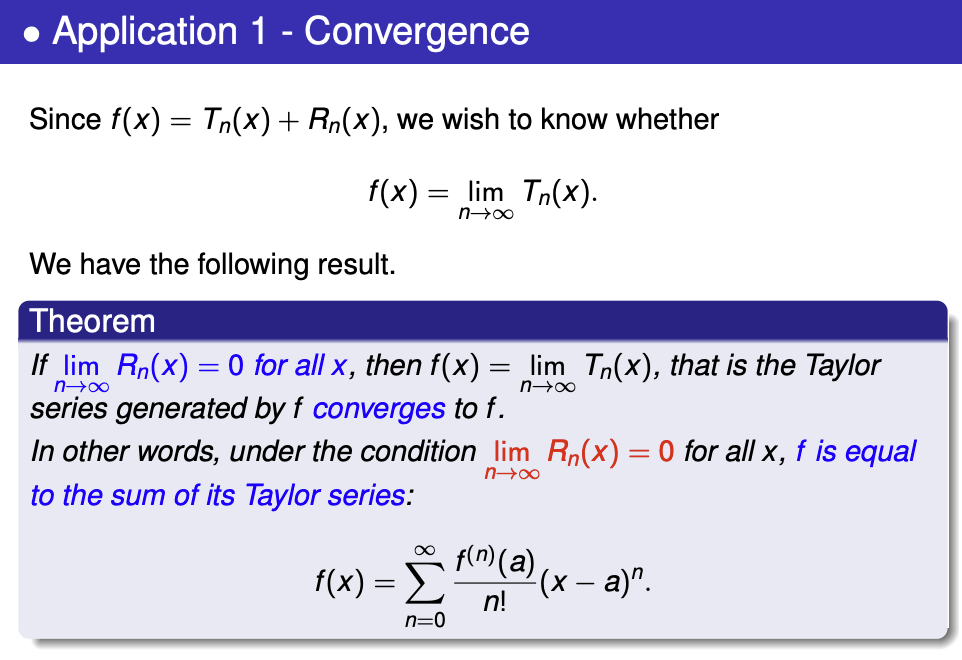
\includegraphics[scale=0.7]{appli 1-convergence.png}
\end{center}
In other word, given a function, you first write the Taylor remainder of the Taylor series generated by this function. After that, you should determine the limit of this remainder.  \\ \\ 
\textbf{Example.} Show that the Taylor series for cos x at $x=0$ converges to cos x for every value of x. \\ \\ 
\textit{Solution. } We add the remainder term to the Taylor polynomial for cos x to obtain Taylor’s formula for cos x with $n = 2k$:
$$ \cos x =  1 - \frac{x^2}{2!} + \frac{x^4}{4!} - ... + (-1)^k \frac{x^{2k}}{(2k)!}+ R_{2k}(x) $$
Because the derivatives of the cosine have absolute value less than or equal to 1, the
Remainder Estimation Theorem with $M = 1$ gives:
$$ |R_{2k}(x)| \leq 1 \cdot \frac{|x|^{2k+1}}{(2k+1)!}$$
For every value of x, $R_{2k} \to 0$ as $k \to \infty$. Therefore, the series converges to cos x for every value of $x$. Thus,
$$ \cos x = \sum_{k=0}^{\infty} \frac{(-1)^k x^{2k}}{(2k)!} = 1 - \frac{x^2}{2!} + \frac{x^4}{4!} - \frac{x^6}{6!} + ...$$
\subsubsection{Error Estimation}
\begin{center}
        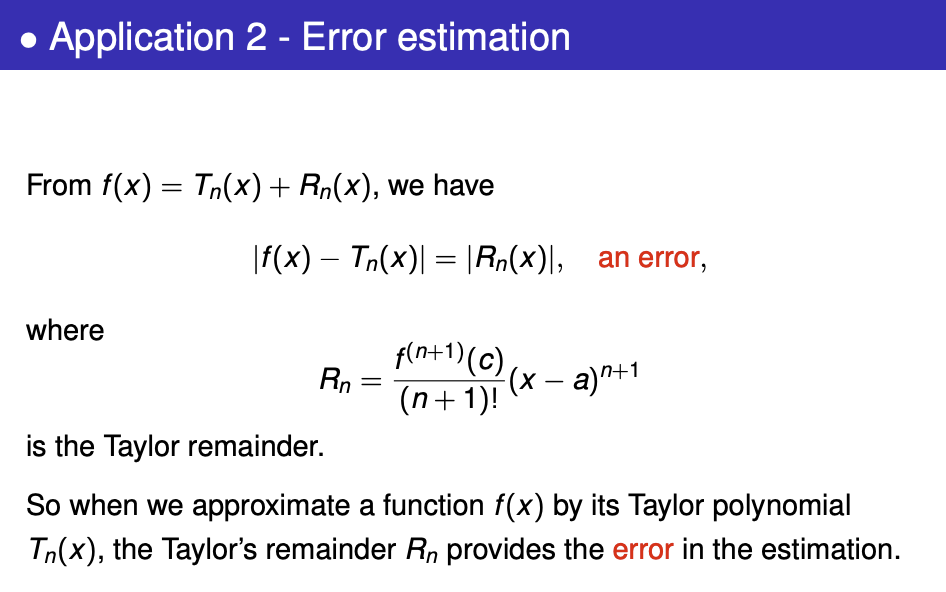
\includegraphics[scale = 0.7]{application 2. error estimation.png}
\end{center}
\textbf{Example. } Estimate the value if $P_4(x) =  1 + x + (x^2/2) + (x^3/6) + (x^4/24)$ is used to estimate the value of $e^x$ at $x=1/2$. \\ \\
\textit{Solution} Recognize that $P_4(x)$ is the Taylor polynomials of $e^x$ at degree 4.  Recall that when we approximate a function $f(x)$ by its Taylor polynomial $T_n(x)$, the Taylor’s remainder $R_n$ provides the error in the estimation. \\ \\
Therefore, the error if $P_4(x)$ is used to estimate $e^x$ at $x=1/2$ is:
\begin{align*}
    R_4(x) &=  \frac{f^{(n+1)}(c)}{(n+1)!} (x-a)^{n+1} \text{ for n = 4 in our exercise.} \\
    &= \frac{f^{(5)}(c)}{5!} (0.5)^{4+1} \\
    &= \frac{e^c}{5!}(0.5)^5
\end{align*}
 For $c \in [0, 0.5], e^c \leq e^{0.5}$ or $e^c \leq 2.7$
 The error is: 
 $$ R_4 \leq 7.03 \cdot 10^{-4} $$

\textbf{Extra Notes.} You may take a look at the Alternating Series Estimation Theorem to deal with these exercises: 
\begin{center}
        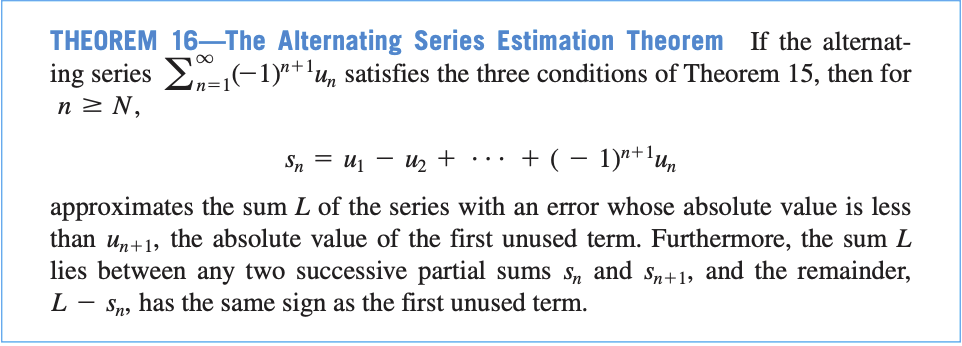
\includegraphics[scale = 0.7]{additional theorem.png}
\end{center}

\end{document}
